% !TeX root = ../main.tex
% %%%%%%%%%%%%%%%%%%%%%%%%%%%%%%%%%%%%%%%%%%%%%%%%%%%%%%%%%%%%%%%%%%%%%%%%%%%%%%
% Introduction
\chapter{Introduction}
\label{chap:introduction}

This thesis aims to explore a possible solution for automation in the testing of robotic systems through a domain-specific language (DSL) and simulation-based monitoring software.

A DSL is a programming language that is written for a specific domain, it usually provides a higher level of abstraction and is simpler than other languages mainly because they are intended to be used by people knowledgeable of the domain.

This chapter intends to introduce the motivation for this work (\autoref{sec:motivation}), present the problem statements of such an approach (\autoref{sec:problem}), discuss the objectives (\autoref{sec:objectives}), show a motivational example of the developed work (\autoref{sec:motivationalexample}), present the expected contributions (\autoref{sec:contributions}), and finally summarize the structure of the rest of the document (\autoref{sec:structure}).


% ------------------------------------------------------------------------------
% Motivation
\section{Motivation}
\label{sec:motivation}

Robotics already significantly impact our current society, in industry, in medicine, in agriculture, or leisurely in sports contests or personal use. Robotics often take critical roles like the example of robot arms in car assembly lines or autonomous farms. The tendency is for robot usage to keep growing at a global level. 

Robotic Systems are non-deterministic, mainly because robots interact directly with the real world. Testing software in such environments is complex, as many variables can change, and verifying the success of a task or movement may not be possible from the robot's perspective, and external monitoring may be required.

Current practices in testing robot software mainly involve field testing, simulation testing, and log checking and require a human to analyze the robot's behavior to determine whether the behavior is correct. Due to their broad practicality, the quality of software running on robots should be extremely important to us. Robot software, as well as the techniques used to test their quality, are very field-specific and different from the techniques employed in traditional Software Engineering mainly because of their real-world interaction. This peculiarity means automatic tests are rarely used in robotics~\cite{9240632,zizyte2021importance}.

Studying possible options for viable automation of tests in robotic systems could lead to an opening on its usage in both research and the industry. Also, allowing for multiple parallel executions of tests not depending on human monitoring could improve the quality of current and future robot software.


% ------------------------------------------------------------------------------
% Problem Statement
\section{Problem Statement}
\label{sec:problem}

The multiple challenges in robot testing influence the planning for testing a robot because there are tradeoffs among choices.

Using simulation-based testing, developers can take advantage of real values of objects' attributes to compare with what the robot system perceives. Using this alleyway, it is possible to, in a way, surpassing the need for human-in-the-loop testing.

Human-in-the-loop testing refers to a method of testing that requires a human to perform a certain task that can't be covered by means of automation or simulation.
 
While simulation-based tests are a promising approach for automation, there is still distrust in the precision and validity of the results. As a result, simulation-based autonomous testing is rarely used due to reliability and factors like cost and complexity~\cite{9240632,zizyte2021importance}.
Due to these factors, despite being dangerous, sometimes expensive, or work-intensive, real-life robot testing or other methods are still the main choices. The resulting product is a lack of quality in the software across projects.

In this thesis, I address problems of defining simulation-based automated tests for robotics systems.


% ------------------------------------------------------------------------------
% Objectives
\section{Objectives}
\label{sec:objectives}

The ultimate goal of this thesis is to remove the need for human-in-the-loop testing of robotic systems by studying a possible solution for automation in simulation-based tests.

This work aims to provide developers with a way to verify their robotic systems' properties in relation to their position in a simulation (positional properties) aswell as correlations between current and past events (temporal properties). To this end, I propose the introduction of a DSL for developers to express their relevant properties. The given properties compile into monitors that can be used in simulation to ensure the correctness of the system. The DSL was designed from the point of view of the Robot Operating System (ROS)~\cite{quigley2009ros} developers and tries to abstract the underlying Linear Temporal Logic (LTL) system. LTL is a branch of logic responsible for representing and reasoning about modalities in reference to time. The DSL allows properties to reason about native ROS constructs, like \textit{topics}, \textit{messages} and simulation information. Thus, it is possible to express properties that relate the internal information of the system with the corresponding information in the simulator.

The DSL should allow describing a robotic system's properties simply and intuitively while simultaneously expressing relevant temporal and positional arguments between robots components and objects in the simulation. For this reason, the expected design goals of the DSL that I believe conform with ROS developers are:

\begin{itemize}
\item Temporal operators based on but not restricted to Linear Temporal Logic.
\item Primitives to make references to the simulation environment, like the position, velocity, or any others.
\item Basic operators to make comparisons between defined components, like greater than, equals, and others.
\end{itemize}


% ------------------------------------------------------------------------------
% Motivational Example
\section{Motivational Example}
\label{sec:motivationalexample}

Let us consider an autonomous car developer wanting to express that the car always stops when near a stop sign. The following example presents a property defined in the language that specifies the intended behavior of the developer.

\texttt{after\_until robot.distance.stop\_sign < 1, robot.distance.stop\_sign > 1, eventually robot.velocity == 0}

\textit{Translating into natural language, the property states in the first section that after the robot's distance to the stop-sign is below the value of 1 in the simulator, and in the second section that up until the distance is again above 1, then in the third section the robot velocity will eventually be equal to 0.}

The toolchain compiles the DSL specification to executable Python code that is capable of running as a ROS node. The node listens only to relevant topics and performs the computations to verify the specified property.

\begin{figure}
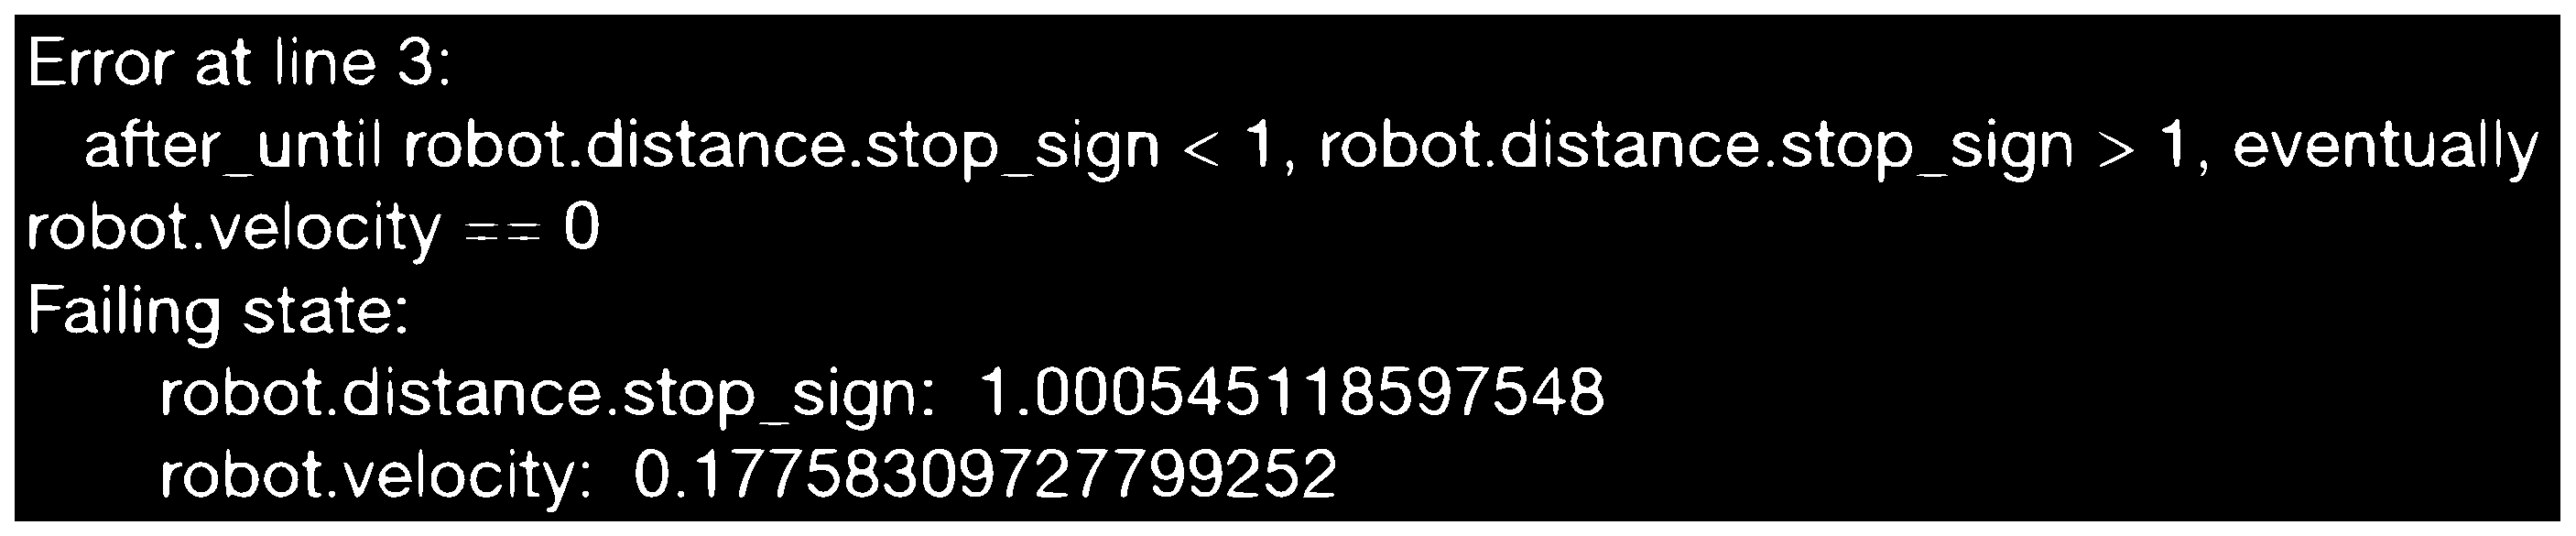
\includegraphics[width=\textwidth]{images/error.eps}
\caption{Example of the displayed error when the robot does not stop at the stop sign.} \label{fig:error}
\end{figure}

The flow of the process of monitoring a robotic system is described as follows:

\begin{enumerate}[label=(\roman*)]
    \item \textbf{Property formalization:} The developer describes in the DSL the properties of the robotic system one wants to monitor in a \texttt{.txt} file extension.
    \item \textbf{Compilation:} The specified properties are compiled, and a python file is generated capable of running as a ROS node.
    \item \textbf{Monitoring:} The node can be run whenever testing the system and will listen to pertinent topics and perform the computations needed to verify the specified properties.
\end{enumerate}


% ------------------------------------------------------------------------------
% Contributions
\section{Contributions}
\label{sec:contributions}

The expected contributions of this thesis are below enumerated.

\begin{enumerate}
    \item Definition of a domain-specific language to specify robotic systems' properties.
    \item Implementation of a compiler for the language that can generate software capable of monitoring relevant components while in a simulation.
    \item Evaluation of the expressive capabilities of the solution.
\end{enumerate}


% ------------------------------------------------------------------------------
% Structure of the document
\section{Structure of the document}
\label{sec:structure}

The document is organized as follows:

\begin{itemize}
    \item \autoref{chap:background} - Background \& Related Work:
    \item \autoref{chap:language} - Specification Language for Robotics Properties
    \item \autoref{chap:monitoring} - Monitoring
    \item \autoref{chap:evaluation} - Evaluation 
    \item \autoref{chap:futurework} - Future Work
    \item \autoref{chap:conclusion} - Conclusion
\end{itemize}
